\documentclass[11pt,a4paper,sans]{moderncv}

% moderncv themes
\moderncvstyle{banking}                            % style options are 'casual' (default), 'classic', 'oldstyle' and 'banking'

\moderncvcolor{blue}                                % color options 'blue' (default), 'orange', 'green', 'red', 'purple', 'grey' and 'black'

%\renewcommand{\familydefault}{\sfdefault}         % to set the default font; use '\sfdefault' for the default sans serif font, '\rmdefault' for the default roman one, or any tex font name

%\nopagenumbers{}                                  % uncomment to suppress automatic page numbering for CVs longer than one page

% character encoding
\usepackage[utf8]{inputenc}                       % if you are not using xelatex ou lualatex, replace by the encoding you are using

% adjust the page margins
\usepackage[scale=0.75]{geometry}

\usepackage{natbib}
\usepackage{graphicx}

%  to redefine the heading string ("Publications"):
\renewcommand{\refname}{Working Papers}
\newcommand\mybitem[1]{%
   \parbox[t]{3mm}{\textbullet}\parbox[t]{10cm}{#1}\\[1.6mm]}

%\setlength{\hintscolumnwidth}{3cm}                % if you want to change the width of the column with the dates

%\setlength{\makecvtitlenamewidth}{10cm}           % for the 'classic' style, if you want to force the width allocated to your name and avoid line breaks. be careful though, the length is normally calculated to avoid any overlap with your personal info; use this at your own typographical risks...

% personal data
\name{Elisha}{Cohen}
%\title{Resumé title}                               % optional, remove / comment the line if not wanted
\address{PhD Student, Demography and Social Policy}{Office of Population Research}{Princeton University}% optional, remove / comment the line if not wanted; the "postcode city" and and "country" arguments can be omitted or provided empty
%\phone[mobile]{+1~(917)~334~3844}                   % optional, remove / comment the line if not wanted
%\phone[fixed]{+2~(345)~678~901}                    % optional, remove / comment the line if not wanted
%\phone[fax]{+3~(456)~789~012}                      % optional, remove / comment the line if not wanted
\email{cohen dot elisha at gmail dot com}                       % optional, remove / comment the line if not wanted
\homepage{http://ecohen13.github.io/}                         % optional, remove / comment the line if not wanted
%\extrainfo{additional information}                 % optional, remove / comment the line if not wanted
%\photo[64pt][0.4pt]{picture}                       % optional, remove / comment the line if not wanted; '64pt' is the height the picture must be resized to, 0.4pt is the thickness of the frame around it (put it to 0pt for no frame) and 'picture' is the name of the picture file
%\quote{Some quote}                                 % optional, remove / comment the line if not wanted

% to show numerical labels in the bibliography (default is to show no labels); only useful if you make citations in your resume
%\makeatletter
%\renewcommand*{\bibliographyitemlabel}{\@biblabel{\arabic{enumiv}}}
%\makeatother
%\renewcommand*{\bibliographyitemlabel}{[\arabic{enumiv}]}% CONSIDER REPLACING THE ABOVE BY THIS

% bibliography with mutiple entries
%\usepackage{multibib}
%\newcites{book,misc}{{Books},{Others}}
%----------------------------------------------------------------------------------
%            content
%----------------------------------------------------------------------------------
\begin{document}
%\begin{CJK*}{UTF8}{gbsn}                          % to typeset your resume in Chinese using CJK
%-----       resume       ---------------------------------------------------------
\makecvtitle
%% -----------------------------------------------------------
%% Research Interests
%% -----------------------------------------------------------
\section{Research Interests}
Quantitative methods and approaches of causal inference for social policy.
%% -----------------------------------------------------------
%% Education
%% -----------------------------------------------------------
\section{Education}
\cventry{2013--}{In Progress -- PhD in Demography and Social Policy}{Office of Population Research, Princeton University}{Princeton, NJ}{\textit{}}{}
\cventry{2012}{Master of Arts in Economics}{Hunter College, CUNY}{New York, NY}{\textit{}}{}  % arguments 3 to 6 can be left empty

\cventry{2003}{Bachelor of Arts in Economics}{University of Wisconsin - Madison}{Madison, WI}{\textit{}}{}

%% -----------------------------------------------------------
%% Teaching
%% -----------------------------------------------------------
\section{Teaching Experience}
\cventry{}{}{Princeton University}{Princeton, NJ}{}{}
\vspace{-5mm}
\begin{itemize}
	\item{\emph{Assistant Instructor, SOC 504: Advanced Social Statistics, Graduate Course \hspace{11mm}Spring 2016} \newline Course Head: Brandon Stewart, Asst. Prof. of Sociology}
	\item{\emph{Instructor, Statistical Programming Camp, Graduate Course \hspace{33mm} January 2016}\newline Course Head: Kosuke Imai, Prof. of Politics}
	\item{Assistant Instructor, SOC 500: Applied Social Statistics, Graduate Course \hspace{19mm}Fall 2015 \newline Course Head: Brandon Stewart, Asst. Prof. of Sociology}
	\item{Assistant Instructor, POL 245: Visualizing Data, Freshman Scholars Institute \hspace{8mm}Summer 2015 \newline Course Head: Kosuke Imai, Prof. of Politics}
\end{itemize}
\cventry{}{}{Hunter College - CUNY}{New York, NY}{}{}
\vspace{-5mm}
\begin{itemize}
	\item{\emph{Teaching Assistant, Principles of Economics: Microeconomics, \hspace{37mm}Fall 2012} \newline \emph{Undergraduate Course} \newline Course Head: Howard Chernick, Prof. of Economics}
	\item{\emph{Tutoring, Statistics and Programming in Stata} \hspace{40mm}May 2012 - August 2013}
\end{itemize}
%% -----------------------------------------------------------
%% Working Papers
%% -----------------------------------------------------------
\section{Working Papers}
\cvitem{Health and Aging Trends of Elderly Mexican-Americans in the United States}{Elisha Cohen}
\cvitem{Analyzing the Causal Path to Infant Mortality: the Mediating Effect of Low Birthweight}{Elisha Cohen}
\cvitem{The Effect of Massachusetts Health Care Reform on the Rate of Preventable Hospitalizations}{Elisha Cohen, Partha Deb, Rebecca Gorges, and Ruirui Sun.}
\cvitem{The Medicaid Effect: Do Medicaid Patients have More Low Birthweight Infants?}{Master's Thesis, Advisor: Prof. Partha Deb}
%% -----------------------------------------------------------
%% Working Papers
%% -----------------------------------------------------------
% Publications from a BibTeX file without multibib
%  for numerical labels: \renewcommand{\bibliographyitemlabel}{\@biblabel{\arabic{enumiv}}}% CONSIDER MERGING WITH PREAMBLE PART
%  to redefine the heading string ("Publications"): \renewcommand{\refname}{Articles}
\nocite{*}
\bibliographystyle{plain}
\bibliography{publications}                        % 'publications' is the name of a BibTeX file

% Publications from a BibTeX file using the multibib package
%\section{Publications}
%\nocitebook{book1,book2}
%\bibliographystylebook{plain}
%\bibliographybook{publications}                   % 'publications' is the name of a BibTeX file
%\nocitemisc{misc1,misc2,misc3}
%\bibliographystylemisc{plain}
%\bibliographymisc{publications}                   % 'publications' is the name of a BibTeX file

%% -----------------------------------------------------------
%% Work Experience
%% -----------------------------------------------------------
\section{Research Experience}
%\subsection{Vocational}
\cventry{2013}{Research Assistant}{Dr. Partha Deb, CUNY}{New York, NY}{}{Collaborated with the Visiting Nurse Service of New York's Center for Home Care Policy and Research on a Heart Failure Study. Programmed (in Stata) to process raw data, perform data cleaning and run statistical analysis using methods such as instrumental variable regression.}
\cventry{2013}{Research Assistant}{Dr. Sherry Glied, Columbia University}{New York City, NY}{}{Programmed in Stata to create propensity score anlaysis for evaluation of disability and health outcomes.}
%% -----------------------------------------------------------
%% Conferences
%% -----------------------------------------------------------
\section{Conference Presentations}
\cvitem{Population Association of America, 2015}{Health Differentials of Older Hispanic Immigrants by Visa Status and Age}
\cvitem{International Conference on Aging in the Americas, 2014}{Health Differentials of Older Hispanic Immigrants by Age at Arrival}
\cvitem{New York State Economics Association, 2012}{The Effect of Massachusetts Health Care Reform on the Rate of Preventable Hospitalizations}
%% -----------------------------------------------------------
%% Awards
%% -----------------------------------------------------------
\section{Awards}
\cvitem{Princeton University Fellowship 2013-2016}{}
\cvitem{Certificate of Academic Achievement in Economics}{Hunter College, CUNY}
% \section{Languages}
% \cvitemwithcomment{English}{Skill level}{Comment}
% \cvitemwithcomment{Language 2}{Skill level}{Comment}
% \cvitemwithcomment{Language 3}{Skill level}{Comment}

\section{Computer skills}
\subsection{Programming}
\cvdoubleitem{Advanced}{R, Stata}{Beginner}{Python}
\subsection{R Packages}{\url{https://github.com/ecohen13}}
\subsection{Software}
\cvdoubleitem{Typesetting}{\LaTeX}{Version Control}{Git, Subversion}
\cvdoubleitem{Database}{Microsoft Access}{}{}
%\cvdoubleitem{Programming}{R(advanced), Stata(advanced), Python(beginner)}{}{}
%\cvdoubleitem{Typsetting}{Latex}{}{}

\section{Service}
\cvitem{OPR Student Wiki}{Administrator 2014-2016}
\cvitem{OPR Graduate Student Professional Development Committee}{Co-chair 2014-2015}
\cvitem{Graduate Student Government}{PIPS/JDP Representative 2013-2014}

% \section{Interests}
% \cvitem{hobby 1}{Description}
% \cvitem{hobby 2}{Description}
% \cvitem{hobby 3}{Description}

% \section{Extra 1}
% \cvlistitem{Item 1}
% \cvlistitem{Item 2}
% \cvlistitem{Item 3. This item is particularly long and therefore normally spans over several lines. Did you notice the indentation when the line wraps?}

% \section{Extra 2}
% \cvlistdoubleitem{Item 1}{Item 4}
% \cvlistdoubleitem{Item 2}{Item 5\cite{book1}}
% \cvlistdoubleitem{Item 3}{Item 6. Like item 3 in the single column list before, this item is particularly long to wrap over several lines.}
\section{Coursework -- Princeton University}
\subsection{Quantitative Methods}
\cvitem{POL 501 Quantitative Analysis I}{Fall 2013}
\cvitem{WWS 511D Microeconcomics Analysis (Accelerated)}{Fall 2013}
\cvitem{POL 572 Quantitative Analysis II}{Spring 2014}
\cvitem{POP 502 Research Methods in Demography}{Spring 2014}
\cvitem{POL 573 Quantitative Analysis III}{Fall 2014}
\cvitem{WWS 509 Generalized Linear Statistical Models}{Fall 2014}
\cvitem{POL 574 Quantitative Analysis IV}{Spring 2015}
\cvitem{WWS 598 Epidemiology}{Spring 2015}

\subsection{Field Specific}
\cvitem{POP 501 Survey of Population Problems}{Fall 2013}
\cvitem{WWS 597 The Political Economy of Health Systems}{Fall 2013}
\cvitem{ECO 563 Economic Development II}{Spring 2014}
\cvitem{SOC 506 Research Ethics and Scientific Integrity}{Fall 2014}
\cvitem{WWS 590A Economic Perspectives on Inequality}{Fall 2014}
\cvitem{WWS 590D Psychological Studies of Inequality}{Fall 2014}
\cvitem{WWS 590B Politics of Inequality \& Redistribution}{Spring 2015}
\cvitem{WWS 590C Sociological Studies of Inequality}{Spring 2015}
\cvitem{POP 503 Evaluation of Demographic Research}{Fall 2015}

\section{Student Evaluations}
\subsection{Graduate Students - SOC 500}
\begin{itemize}
	\item ``Elisha is an amazing teacher. Her precepts are always well organized and the material presented in a clear and accessible manner. She is quick to respond to email, and her office hours are always very useful.''
	\item ``Elisha's prepared lessons were great and she was extremely accessible and helpful.''
	\item ``Elisha was particularly excellent at explaining concepts in R and extremely helpful in office hours.''
	\item ``She had a wonderful pace during precept and afterwards I was able to directly connect what we learned to the problem set.''
\end{itemize}
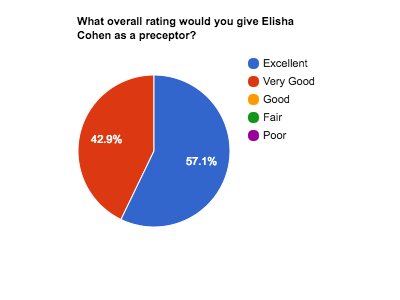
\includegraphics[scale=0.45]{Soc500chart1.png}
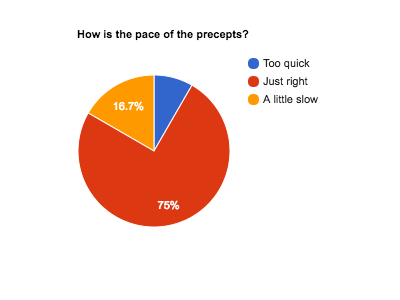
\includegraphics[scale=0.45]{Soc500chart2.png}
\section{References}
\cvitem{Kosuke Imai}{Professor of Politics, Princeton University. \newline email: kimai at princeton.edu}
\cvitem{Brandon Stewart}{Assistant Professor of Sociology, Princeton University. \newline email: brandonmstewart at gmail.com}
\cvitem{Marc Ratkovic}{Assistant Professor of Politics, Princeton University. \newline email: ratkovic at princeton.edu}


\end{document}

